\documentclass[14pt]{extbook}
\usepackage{multicol, enumerate, enumitem, hyperref, color, soul, setspace, parskip, fancyhdr} %General Packages
\usepackage{amssymb, amsthm, amsmath, latexsym, units, mathtools} %Math Packages
\everymath{\displaystyle} %All math in Display Style
% Packages with additional options
\usepackage[headsep=0.5cm,headheight=12pt, left=1 in,right= 1 in,top= 1 in,bottom= 1 in]{geometry}
\usepackage[usenames,dvipsnames]{xcolor}
\usepackage{dashrule}  % Package to use the command below to create lines between items
\newcommand{\litem}[1]{\item#1\hspace*{-1cm}\rule{\textwidth}{0.4pt}}
\pagestyle{fancy}
\lhead{Progress Quiz 5}
\chead{}
\rhead{Version A}
\lfoot{8497-6012}
\cfoot{}
\rfoot{Summer C 2021}
\begin{document}

\begin{enumerate}
\litem{
Solve the rational equation below. Then, choose the interval(s) that the solution(s) belongs to.\[ \frac{-56}{16x -72} + 1 = \frac{-56}{16x -72} \]\begin{enumerate}[label=\Alph*.]
\item \( x_1 \in [-5.5, -1.5] \text{ and } x_2 \in [2.5,5.5] \)
\item \( x \in [-5.5,-1.5] \)
\item \( x \in [3.5,5.5] \)
\item \( x_1 \in [4.5, 6.5] \text{ and } x_2 \in [2.5,5.5] \)
\item \( \text{All solutions lead to invalid or complex values in the equation.} \)

\end{enumerate} }
\litem{
Choose the equation of the function graphed below.
\begin{center}
    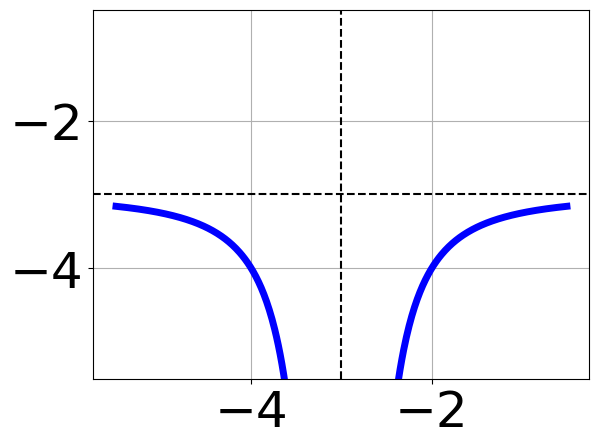
\includegraphics[width=0.5\textwidth]{../Figures/rationalGraphToEquationA.png}
\end{center}
\begin{enumerate}[label=\Alph*.]
\item \( f(x) = \frac{1}{x - 3} - 3 \)
\item \( f(x) = \frac{1}{(x - 3)^2} - 3 \)
\item \( f(x) = \frac{-1}{x + 3} - 3 \)
\item \( f(x) = \frac{-1}{(x + 3)^2} - 3 \)
\item \( \text{None of the above} \)

\end{enumerate} }
\litem{
Choose the equation of the function graphed below.
\begin{center}
    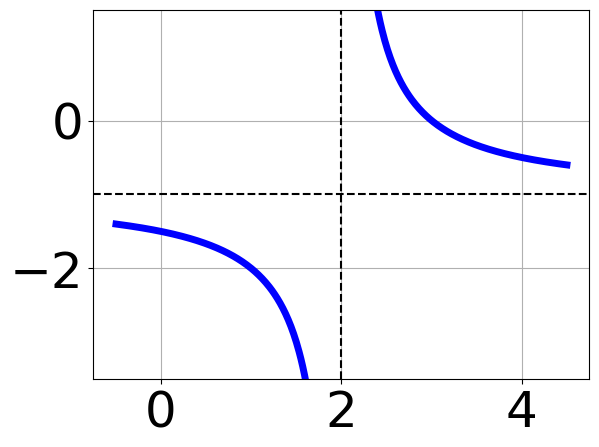
\includegraphics[width=0.5\textwidth]{../Figures/rationalGraphToEquationCopyA.png}
\end{center}
\begin{enumerate}[label=\Alph*.]
\item \( f(x) = \frac{1}{x - 2} - 1 \)
\item \( f(x) = \frac{1}{(x - 2)^2} - 1 \)
\item \( f(x) = \frac{-1}{(x + 2)^2} - 1 \)
\item \( f(x) = \frac{-1}{x + 2} - 1 \)
\item \( \text{None of the above} \)

\end{enumerate} }
\litem{
Choose the graph of the equation below.\[ f(x) = \frac{1}{(x + 3)^2} - 1 \]\begin{enumerate}[label=\Alph*.]
\begin{multicols}{2}\item 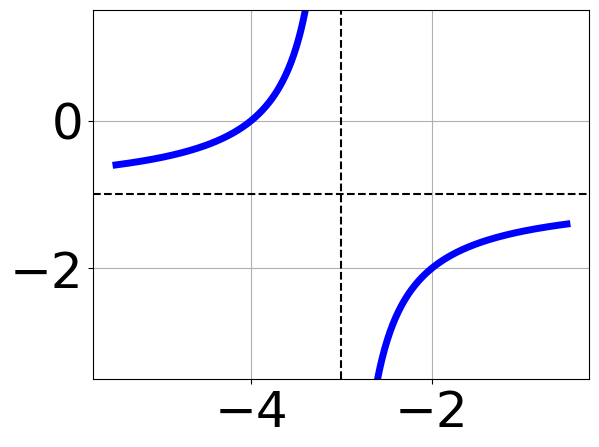
\includegraphics[width = 0.3\textwidth]{../Figures/rationalEquationToGraphCopyAA.png}\item 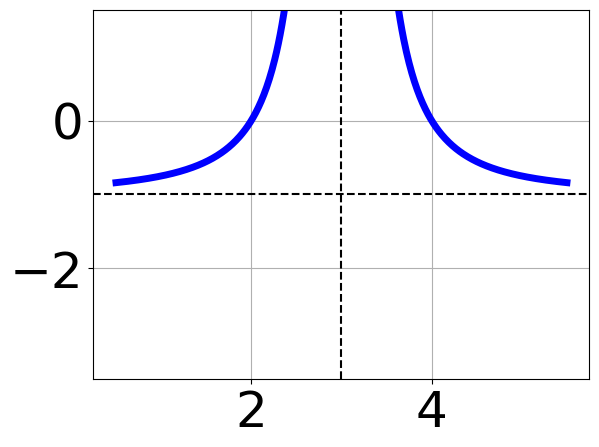
\includegraphics[width = 0.3\textwidth]{../Figures/rationalEquationToGraphCopyBA.png}\item 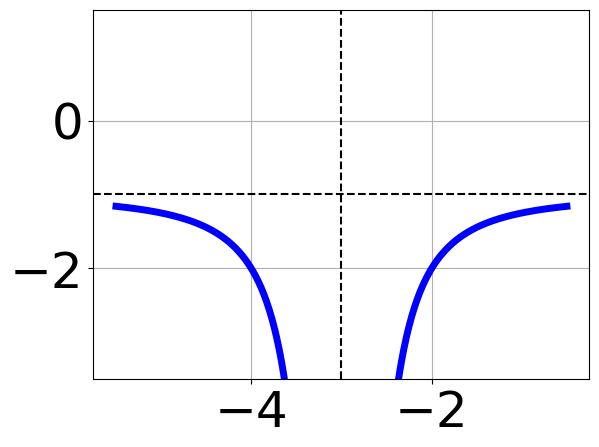
\includegraphics[width = 0.3\textwidth]{../Figures/rationalEquationToGraphCopyCA.png}\item 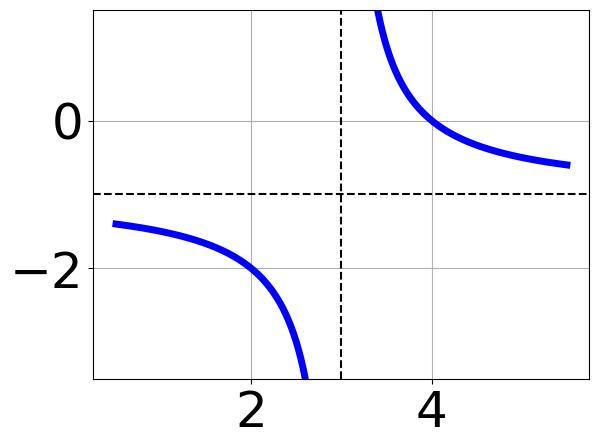
\includegraphics[width = 0.3\textwidth]{../Figures/rationalEquationToGraphCopyDA.png}\end{multicols}\item None of the above.
\end{enumerate} }
\litem{
Solve the rational equation below. Then, choose the interval(s) that the solution(s) belongs to.\[ \frac{-4x}{7x + 6} + \frac{-6x^{2}}{35x^{2} -19 x -42} = \frac{-6}{5x -7} \]\begin{enumerate}[label=\Alph*.]
\item \( x \in [1.53,3.65] \)
\item \( \text{All solutions lead to invalid or complex values in the equation.} \)
\item \( x \in [0.6,1.53] \)
\item \( x_1 \in [-1.34, -0.34] \text{ and } x_2 \in [-3,2.7] \)
\item \( x_1 \in [-1.34, -0.34] \text{ and } x_2 \in [3,6.7] \)

\end{enumerate} }
\litem{
Solve the rational equation below. Then, choose the interval(s) that the solution(s) belongs to.\[ \frac{4x}{4x + 7} + \frac{-2x^{2}}{-8x^{2} +14 x + 49} = \frac{2}{-2x + 7} \]\begin{enumerate}[label=\Alph*.]
\item \( x_1 \in [2.28, 3.46] \text{ and } x_2 \in [-2,3] \)
\item \( x \in [-2.84,-0.99] \)
\item \( x \in [2.68,4.19] \)
\item \( x_1 \in [-2.84, -0.99] \text{ and } x_2 \in [1.5,6.5] \)
\item \( \text{All solutions lead to invalid or complex values in the equation.} \)

\end{enumerate} }
\litem{
Determine the domain of the function below.\[ f(x) = \frac{6}{16x^{2} +40 x + 24} \]\begin{enumerate}[label=\Alph*.]
\item \( \text{All Real numbers except } x = a, \text{ where } a \in [-1.67, -1.4] \)
\item \( \text{All Real numbers except } x = a \text{ and } x = b, \text{ where } a \in [-24.11, -23.87] \text{ and } b \in [-16.78, -15.56] \)
\item \( \text{All Real numbers except } x = a, \text{ where } a \in [-24.11, -23.87] \)
\item \( \text{All Real numbers.} \)
\item \( \text{All Real numbers except } x = a \text{ and } x = b, \text{ where } a \in [-1.67, -1.4] \text{ and } b \in [-1.32, -0.74] \)

\end{enumerate} }
\litem{
Determine the domain of the function below.\[ f(x) = \frac{6}{16x^{2} +8 x -15} \]\begin{enumerate}[label=\Alph*.]
\item \( \text{All Real numbers except } x = a, \text{ where } a \in [-23, -19] \)
\item \( \text{All Real numbers.} \)
\item \( \text{All Real numbers except } x = a, \text{ where } a \in [-4.25, -0.25] \)
\item \( \text{All Real numbers except } x = a \text{ and } x = b, \text{ where } a \in [-23, -19] \text{ and } b \in [12, 13] \)
\item \( \text{All Real numbers except } x = a \text{ and } x = b, \text{ where } a \in [-4.25, -0.25] \text{ and } b \in [0.75, 2.75] \)

\end{enumerate} }
\litem{
Choose the graph of the equation below.\[ f(x) = \frac{-1}{x - 1} + 2 \]\begin{enumerate}[label=\Alph*.]
\begin{multicols}{2}\item 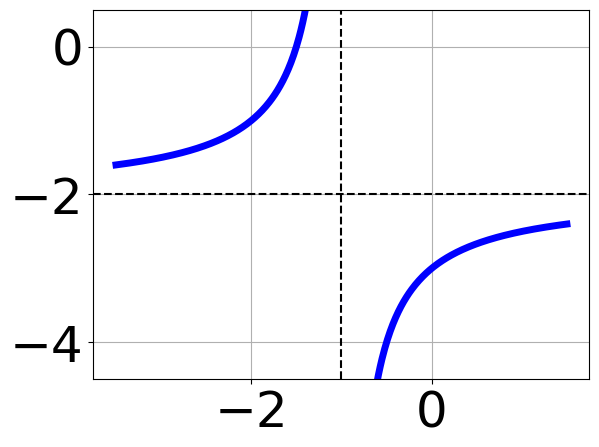
\includegraphics[width = 0.3\textwidth]{../Figures/rationalEquationToGraphAA.png}\item 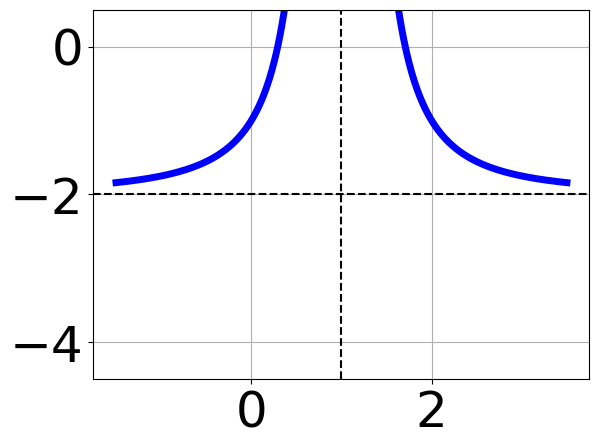
\includegraphics[width = 0.3\textwidth]{../Figures/rationalEquationToGraphBA.png}\item 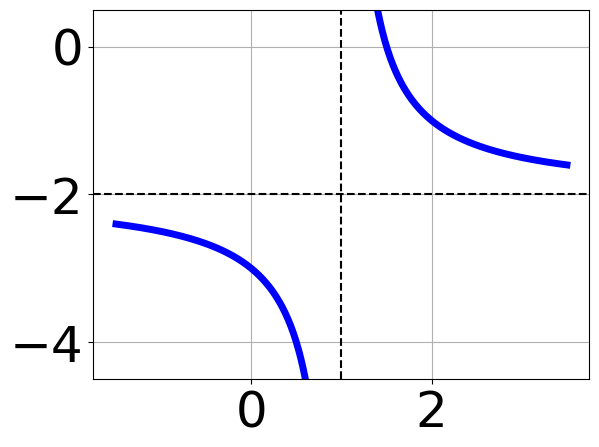
\includegraphics[width = 0.3\textwidth]{../Figures/rationalEquationToGraphCA.png}\item 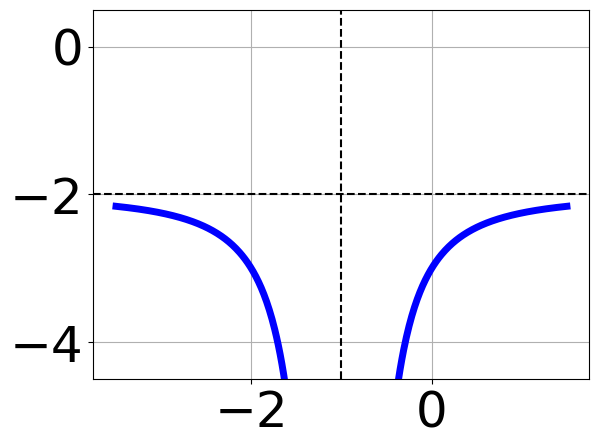
\includegraphics[width = 0.3\textwidth]{../Figures/rationalEquationToGraphDA.png}\end{multicols}\item None of the above.
\end{enumerate} }
\litem{
Solve the rational equation below. Then, choose the interval(s) that the solution(s) belongs to.\[ \frac{108}{72x -36} + 1 = \frac{108}{72x -36} \]\begin{enumerate}[label=\Alph*.]
\item \( x \in [-0.9,-0.2] \)
\item \( x_1 \in [-0.9, -0.2] \text{ and } x_2 \in [-0.5,2.5] \)
\item \( x \in [0.5,2.5] \)
\item \( x_1 \in [0.2, 1.1] \text{ and } x_2 \in [-0.5,2.5] \)
\item \( \text{All solutions lead to invalid or complex values in the equation.} \)

\end{enumerate} }
\end{enumerate}

\end{document}